\documentclass[a4paper,11pt, titlepage]{article}
\usepackage[T1]{fontenc}
\usepackage[english]{babel}
\usepackage{amsmath}
\usepackage{amsfonts}
\usepackage{color}
\usepackage{graphicx}
\usepackage{subfigure}
\usepackage{epsf}
\usepackage[left=2cm,right=2cm,top=2cm,bottom=2cm]{geometry}
\usepackage{float}
\usepackage{lmodern} 
\usepackage[table]{xcolor}
\usepackage{multirow}
\usepackage{listings} 
\usepackage[justification=centering]{caption}
\usepackage{hyperref}
\usepackage[cc]{titlepic}
\usepackage{fancyhdr}
\usepackage{etoolbox}
\usepackage{wrapfig}
\usepackage{booktabs}

%ttfamily

\lstset{% 
language=r, 
basicstyle=\scriptsize, 
keywordstyle=\color{blue}\bfseries, 
commentstyle=\color{black!20!green}, 
stringstyle=\color{red}, 
numbers=left,
numberstyle=\tiny,
frame=\lines
} 

\title{\Huge{Machine learning models for claim prediction in car insurance}}
\author{\Large{Barbara {\sc Gendron-Audebert}}}
\date\today
\titlepic{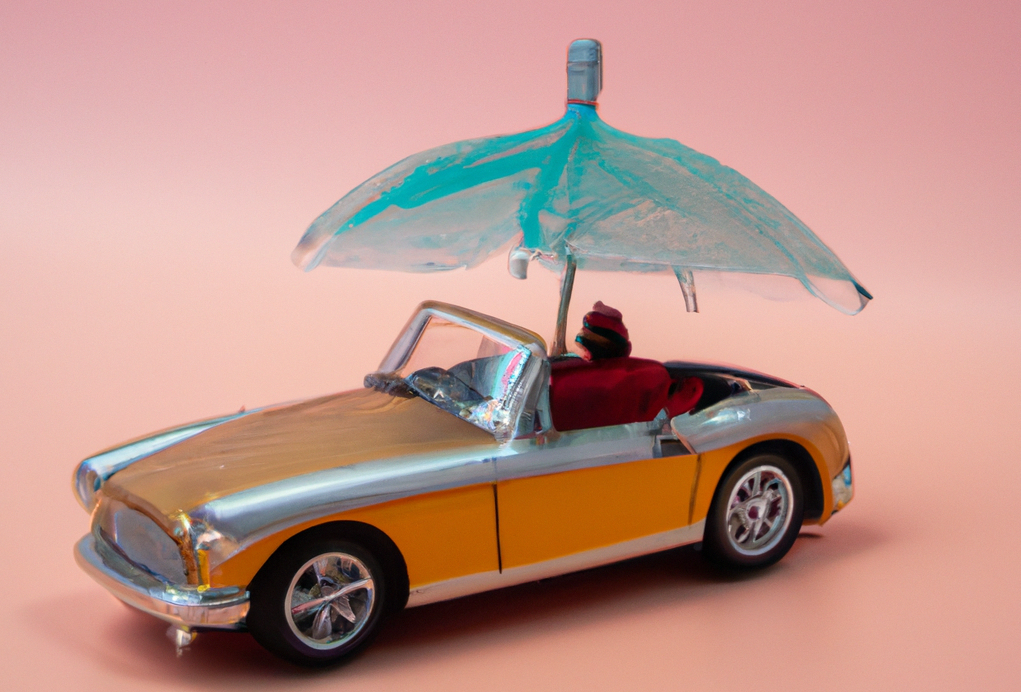
\includegraphics[width=\textwidth]{cover-image.png}}

\patchcmd{\maketitle}
  {\end{titlepage}}
  {\thispagestyle{titlepagestyle}\end{titlepage}}
  {}{}

\fancypagestyle{titlepagestyle}
{
   \fancyhf{}
   \fancyfoot[C]{\emph{A car facing dangers in a hostile planet, protected with an umbrella}, DALL.E generated illustration}
   \renewcommand{\headrulewidth}{0 mm}
}


% --------------------------------------------------------------

\begin{document}
\maketitle
\tableofcontents
\vskip150pt
\section*{Foreword}

This report gives some insights about the use of machine learning techniques in car insurance context. The goal of this work is to leverage data on policyholders related to their driving experience to predict the occurence of a claim. The dataset used to conduct this analysis comes from \href{https://www.kaggle.com/datasets/sagnik1511/car-insurance-data}{this Kaggle page}.\\
\\
In the following sections, we first explore the dataset and describe the related insurance problem in part \ref{data}, before diving in a deeper analysis of the provided features in part \ref{analysis}. In part \ref{models}, one can find insights about the models used to solve this problem, such as a representation of the decision process leading to the model predictions. Finally, part \ref{results} brings a discussion about the provided results, along with some take-aways of this study about car insurance claim prediction.\\
\\
All the technical specifications, the data, all the plots and especially the code (in R) are available in the attached files of the report, and online in \href{https://github.com/B-Gendron/car-insurance-data}{this Git repository}.

\newpage

\section{Data and related insurance problem} \label{data}

\subsection{Dataset description}

The above mentioned dataset contains 19 pieces of information (for now denoted as \textsl{features}) for 10000 policyholders. Among such features, some are closely related to the driving behaviour of the policyholder (driving experience, number of past accidents, \dots), whereas other are more related to its living conditions and family (education, income, \dots). Lastly, the {\tt OUTCOME} feature indicates whether or not the policyholder already experienced a claim. A complete description of the features is given in table \ref{data-description} in the appendix. \\
\\
\noindent If most of the features names are clear enough at first sight, some need to be clarified. The credit score reflect the ability for a policyholder to pay for his debts. The higher the score, the more creditworthy the policyholder is. This parameter has been observed to have a significant influence on the premium in car insurance. The feature {\tt DUIS} refers to DUI, which stands for \textsl{Driving Under the Influence} (whether it be alcohol or drugs).

\subsection{The insurance context}

Machine learning models can be used in the car insurance context for claim prediction by analyzing historical claims data and identifying patterns and trends that can help predict the likelihood of future claims for given policyholders. This can allow insurance companies to better assess risk and price policies accordingly, potentially leading to cost savings for both the insurer and the insured. In this case, the aim is to predict the {\tt OUTCOME} feature from the others, using some machine learning models. 

% -------------------    ANALYSIS    -------------------- % 

\section{Preliminary analysis of the data} \label{analysis}

The purpose of this section is to give a more quantitative description of the data and to go over points of attention to ensure proper modeling.

\subsection{Outliers and missing values}

First, it is usual to compute some basic statistics about each feature on the whole data, such as the minimum and the maximum values, the mean and median. This allows to notice rough anomalies, such as a negative age values. In this dataset, it appears that no anomalies of this type were found.\\
\\
\noindent Descriptive statistics used for this step can be displayed simply using the function {\tt summary()} in R. They are provided along with the number of NA's values for each feature, which corresponds to missing values (NA stands for \textsl{Not Available}). Here, the features {\tt CREDIT SCORE} and {\tt ANNUAL MILEAGE} respectively have 982 and 957 NA's values. This represents approximately 1\% of the whole data for each variable, that's why we can consider simply delete them. Thus, the remaining dataset contains 8149 rows. 

\subsection{Data balance with respect to the {\tt OUTCOME} feature}

Insurance claims are rare events, so there is typically not a lot of data available about them. This limited availability of data on insurance claims can lead to challenges when using machine learning models, as it is well-known that such models require a significant amount of data in order to perform well. Therefore, if the data is too imbalanced with respect to the {\tt OUTCOME} (far more "no" than "yes"), the model won't be able to learn well about the claim, which is precisely the point here. Figure \ref{fig:outcome} shows the value count of 0 and 1, the two possible values for the {\tt OUTCOME} feature. Contrary to what can be expected, claims seem to appear more often that in real life. This would suggest that data was selected on purpose, which implies that no further preprocessing is required on this point. 

\begin{wrapfigure}{r}{6.5cm}
    \centering
    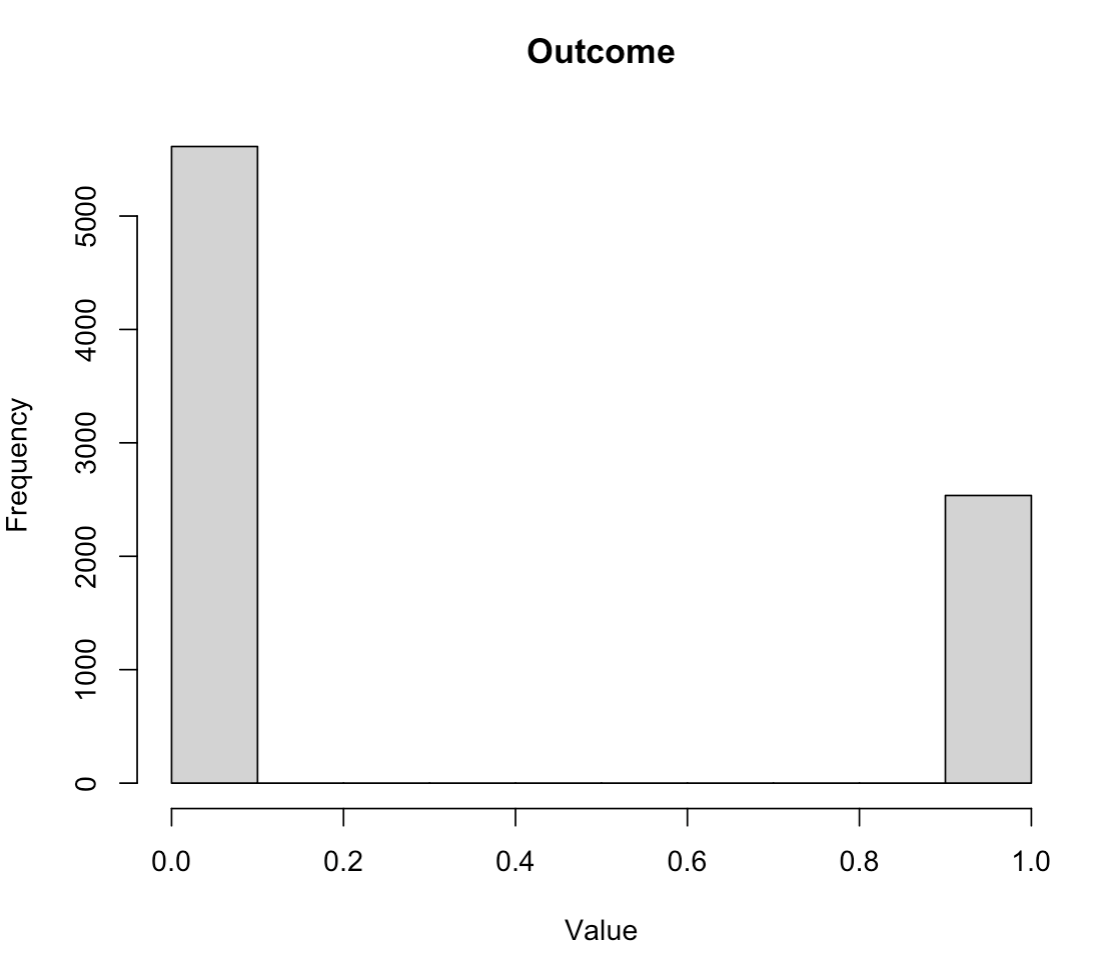
\includegraphics[width=5.5cm]{outcome.png}
    \caption{\centering Distribution of the {\tt OUTCOME} feature.}
    \label{fig:outcome}
\end{wrapfigure}

\subsection{Remaining anomalies in the data}

A fairly important step at this stage would be to check the data for more subtle anomalies, not detected at first glance. One typical way to handle that is to look at the values distribution for each feature and check for relevancy according to what the feature describes in real world. Some plots are provided in the appendix: figure \ref{fig:histograms} shows histograms for quantitative values, whereas figure \ref{fig:categorical-counts} gives the value counts for categorical features with respect to the {\tt OUTCOME} value. This last graph is also useful to check for balance of data, and gives some insights about the relevancy of the features. From this last exploratory data analysis, no further anomalies have been found.\newline

\subsection{Select only the relevant features}

Amongst the 18 features given to describe each policyholder, all are not bound to be helpful when predicted the claim probability. In addition, in order to meet the constraints of the insurance field, some features must be removed because some regulations prohibit their use. This way, let's remove the {\tt GENDER} feature, along with {\tt RACE} for ethical reasons. Now, what remains is to identify the useful features regarding the objective. A typical method for this is to look at the correlation between the {\tt OUTCOME} and the other feature. A correlation coefficient is a number in $[-1,1]$. The higher it is in absolute value, the stronger is the link between the two parameters. Figure \ref{fig:corr} represents the top 10 and flop 10 features most correlated with {\tt OUTCOME}.

\begin{figure}[h!]
    \centering
    \begin{subfigure}
    \centering
    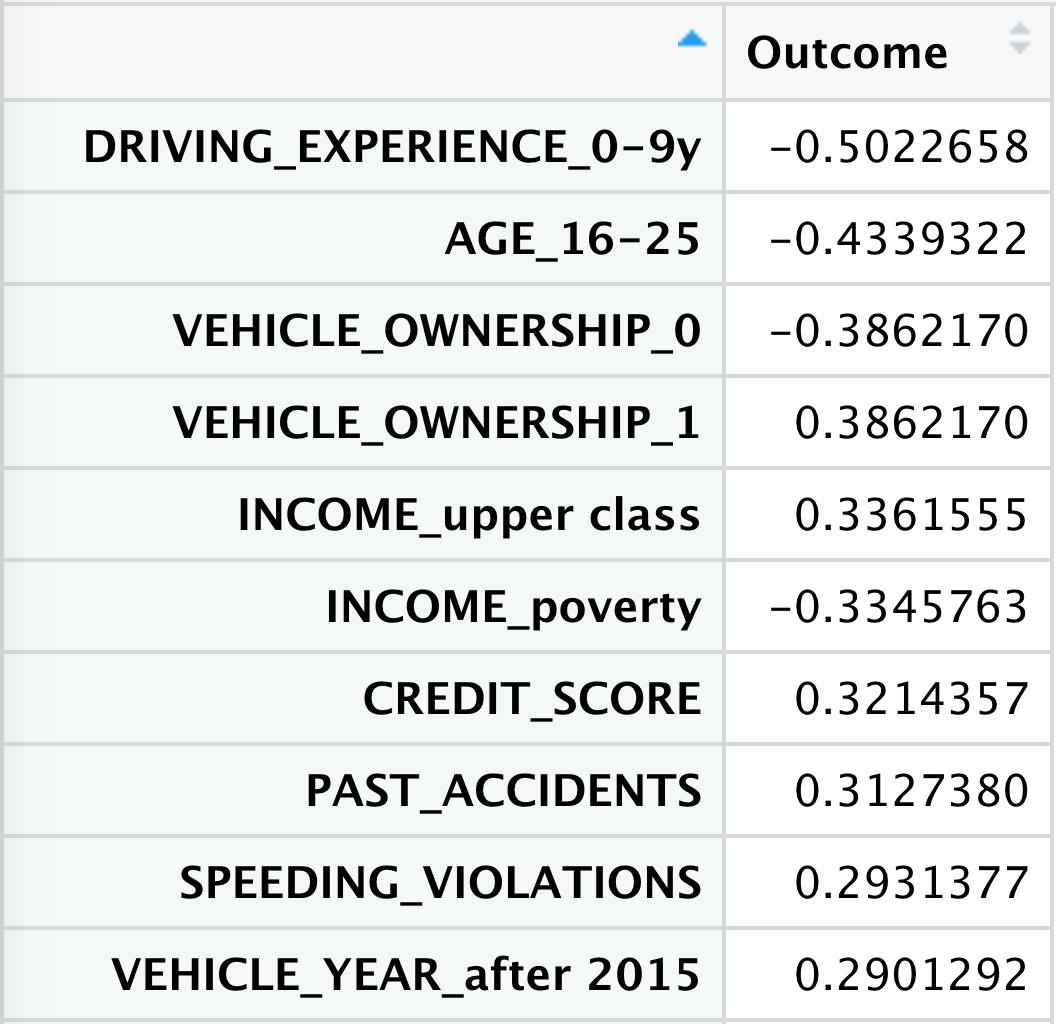
\includegraphics[scale=0.3]{correlations-top10.png}
    \end{subfigure}
    \hskip50pt
    \begin{subfigure}
        \centering
        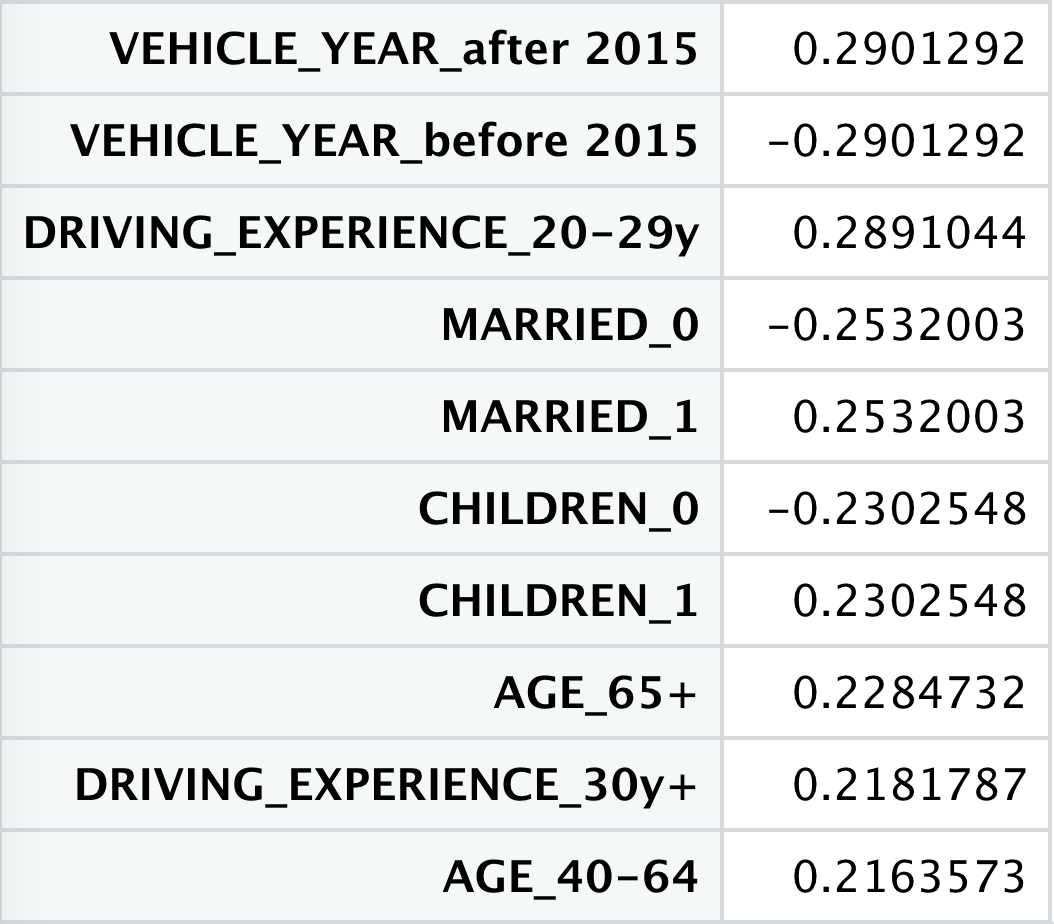
\includegraphics[scale=0.33]{correlations-flop10.png}
    \end{subfigure}
    \caption{\centering Top 10 (left) and flop 10 (right) features most correlated with {\tt OUTCOME}}
    \label{fig:corr}
\end{figure}

\noindent This correlation analysis gives a first insight of which features can be dropped (those that are less correlated with {\tt OUTCOME}). Finally, the dropped features are {\tt GENDER}, {\tt POSTAL\_CODE}, {\tt EDUCATION}, {\tt RACE}, {\tt ID} and {\tt VEHICLE\_TYPE}. Figure \ref{fig:head-data} provides a view of the data after all these steps.\newline

\begin{figure}[h!]
    \centering
    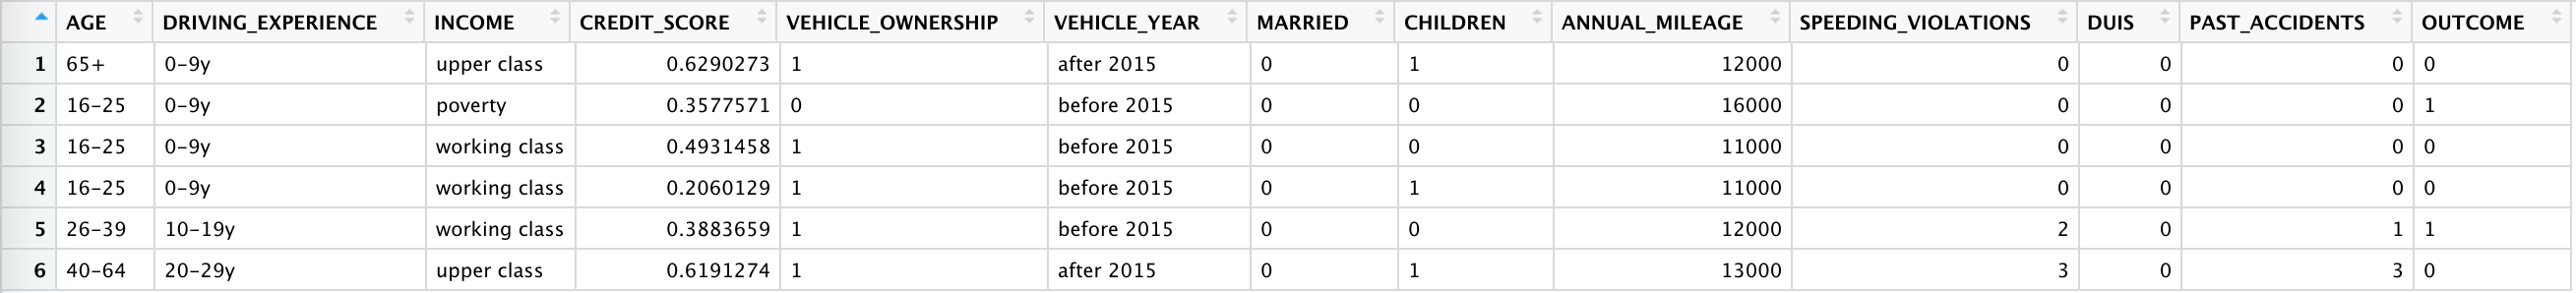
\includegraphics[width=\textwidth]{head-data.png}
    \caption{A view of the 5 first samples of the processed dataset.}
    \label{fig:head-data}
\end{figure}

% -------------------    MODELS    -------------------- % 

\section{Brief description of the models used} \label{models}

This part gives short descriptions of the selected machine learning models for this analysis. The task we need to achieve here is a \textbf{binary classification} (claim or no claim), which is usually handled by the four models to be covered. In order to cover a relevant panel of methods, the following models have been chosen because of their simplicity of structure, their explainability and/or the popularity of such approaches.\\
\\
\noindent Before going through the models, let's define some practical conventions. In the following, "positive" and "1" refer to the outcome \textsl{having a claim}, whereas "negative" and "0" refer to the outcome \textsl{no claim}. 

\subsection{Logistic regression}

Logistic regression is a type of statistical model that is used to predict the probability of an event occurring. Thus, it is a binary classifier. The outcome is modeled as a function of the features which are used to make the prediction of the claim occurence. The term \textsl{logistic} simply refers to the shape of the function used to predict the outcome. Let $f$ be such function and $x$ the representation of the features, the outcome has the following form:
\begin{equation*}
    f(x) = \dfrac{1}{1+e^{-x}}
\end{equation*}

\subsection{Decision tree classifier}

A decision tree classifier is a type of machine learning algorithm that uses a tree-like model to make predictions based on the characteristics or features of an input sample. It works by considering each feature in turn and asking a series of questions about the data, with the goal of identifying the feature or combination of features that best splits the data into classes in a way that maximizes the prediction accuracy. After fitting a decision tree classifier on the data, it is possible to plot the decision tree as it is represented in figure \ref{fig:decision-tree}. For example, this model gives the highest probability of having a claim (0.86) for a driver with less than 10 years of driving experience, who does not own the vehicle and whose vehicle was marketed before 2015.

\begin{figure}[h!]
    \centering
    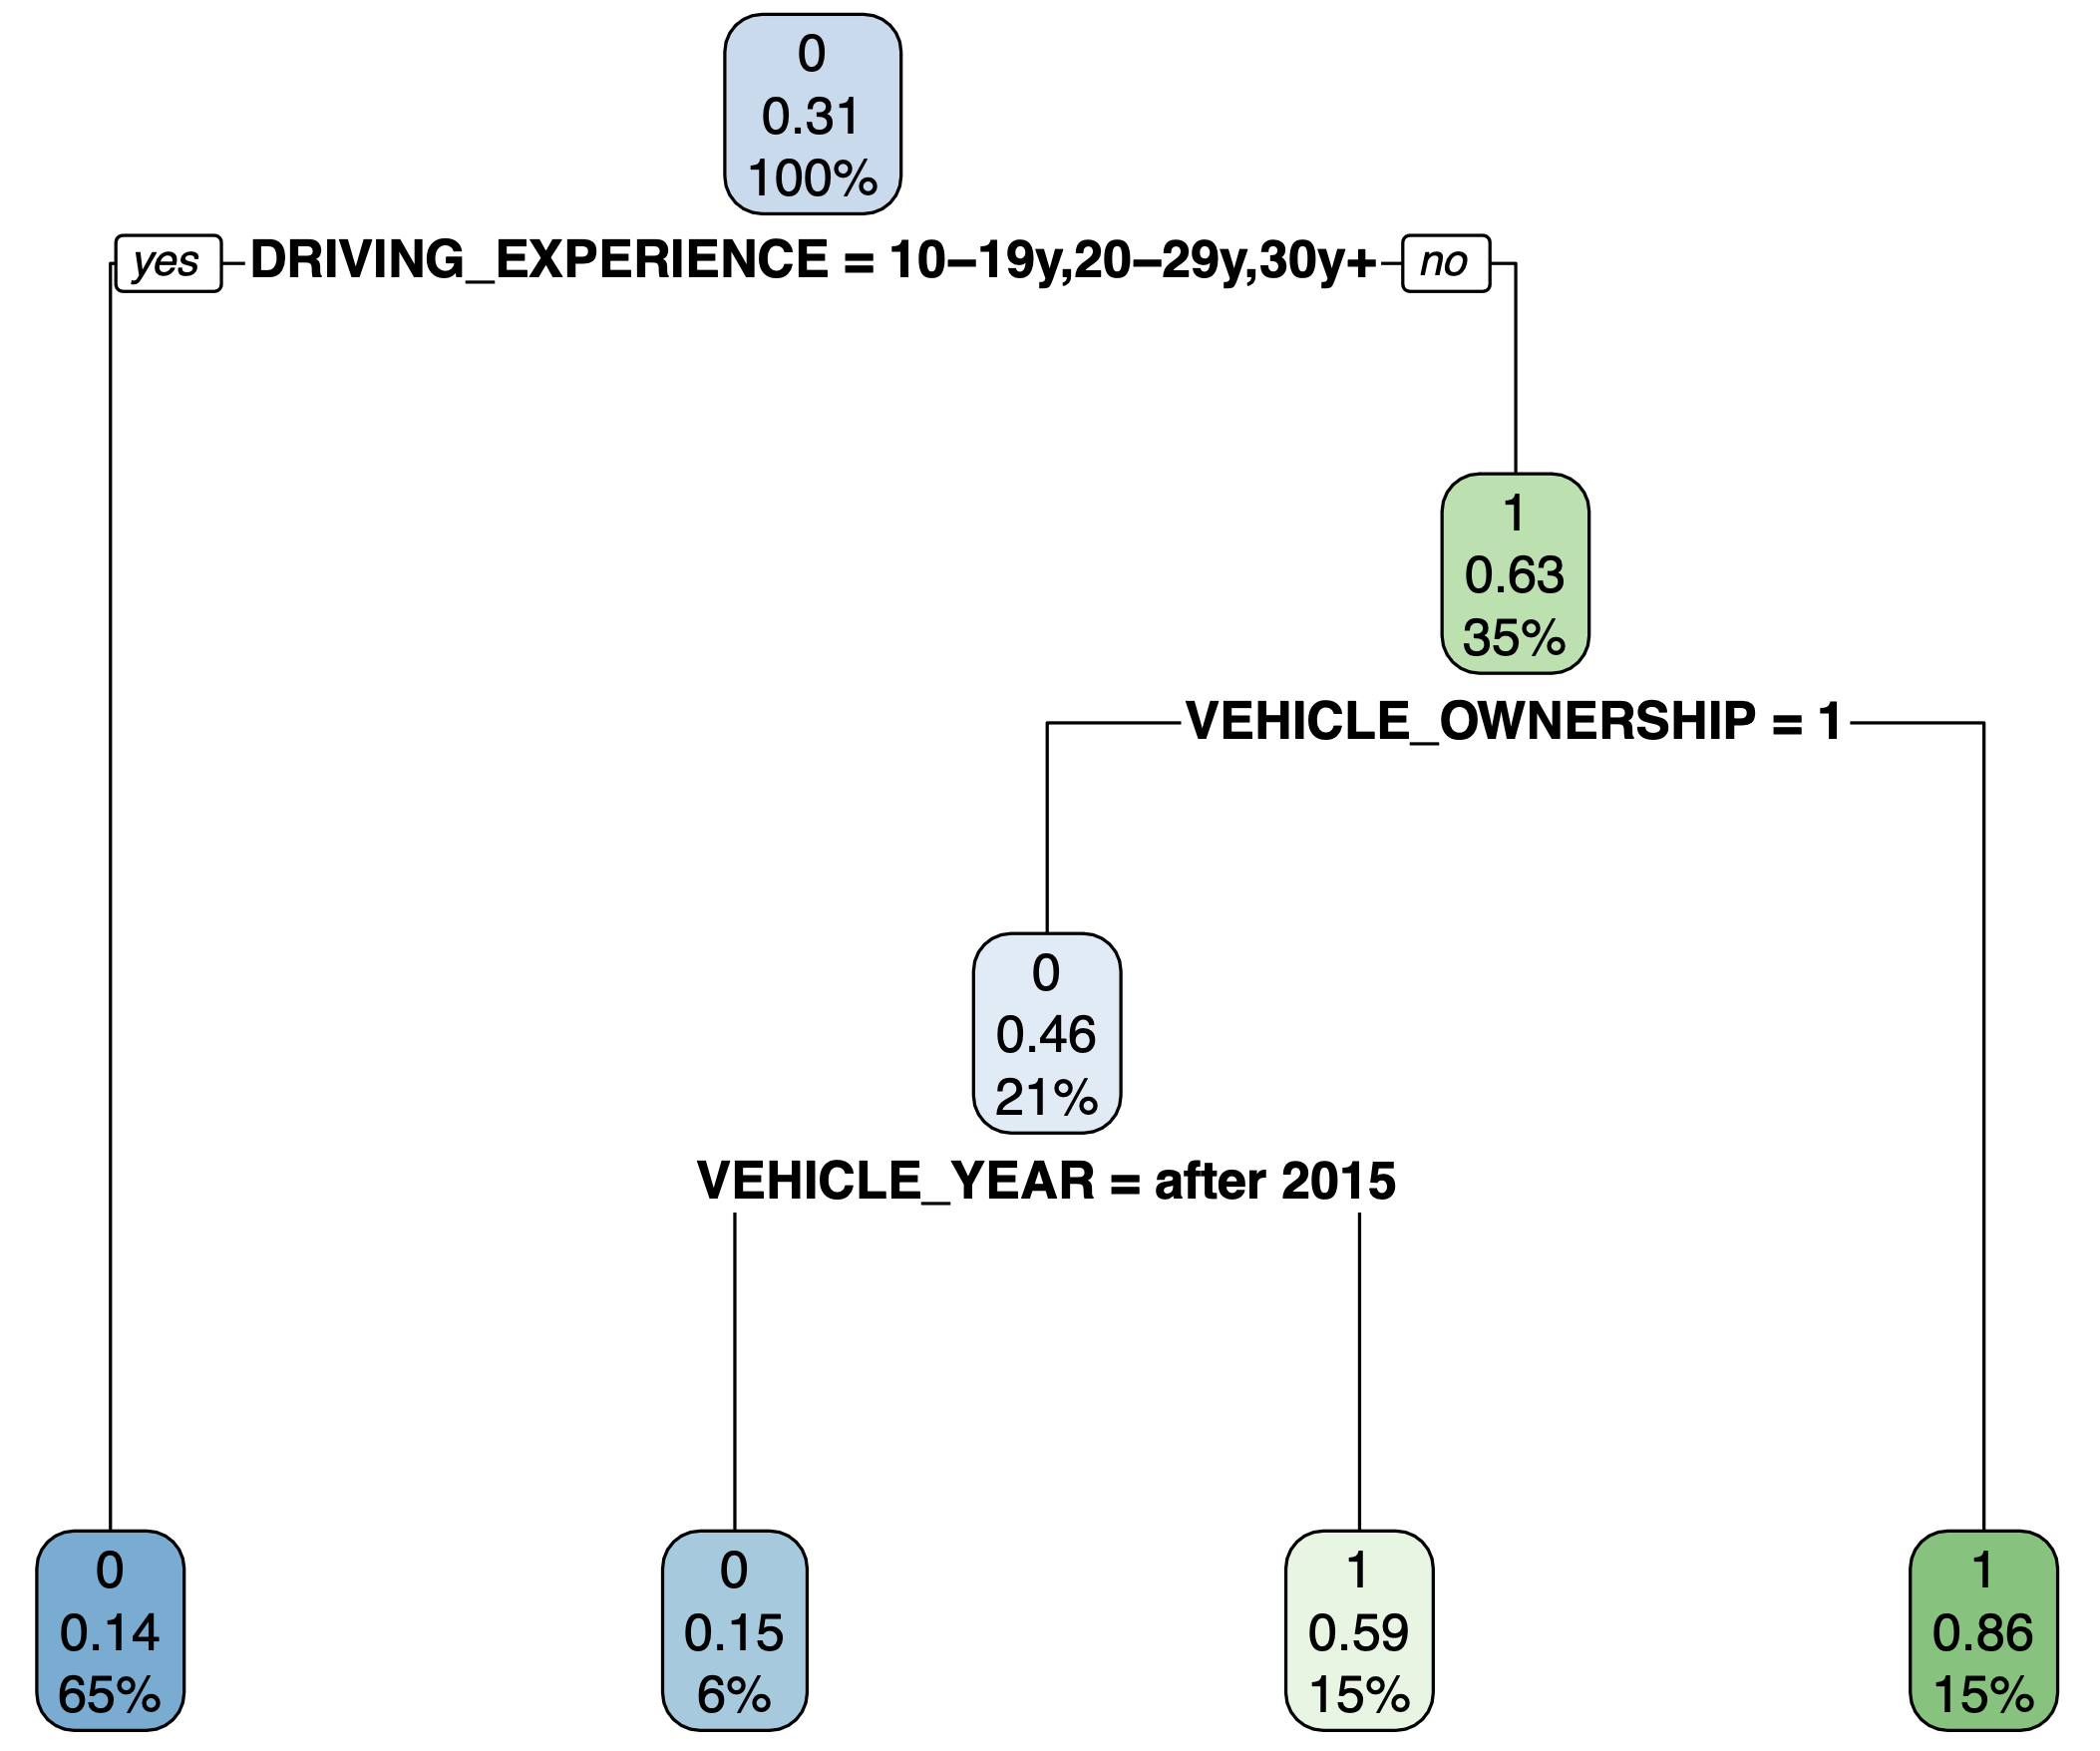
\includegraphics[width=\textwidth]{decision-tree.png}
    \caption{A representation of the decision tree classifier. A positive prediction tend to be pink whereas a negative one tend to be turquoise.}
    \label{fig:decision-tree}
\end{figure}

\subsection{Random forest classifier}

This model is a logical extension of the previous one, in the sense that it contains several decision trees with random initialization. A random forest classifier is often able to make more accurate predictions because it combines the predictions of multiple decision trees, which reduces the variance of the model and helps it to better generalize to new data. 

\subsection{XGBoost}

Finally, XGBoost (eXtreme Gradient Boosting) is a popular and powerful machine learning algorithm. It works by training multiple decision trees in a sequence - contrary to the random forest classifier which train them in parallel, with each tree attempting to correct the errors made by the previous tree. The final model is a weighted average of all the individual decision trees.


% -------------------    RESULTS    -------------------- % 

\section{Analysis of the results and conclusion} \label{results}

\subsection{Training and testing processes}

As the dataset contains the {\tt OUTCOME} value, the binary classficiation task is learnt by the models using \textbf{supervised learning}. The term \textsl{labelled dataset} is therefore used. In supervised learning, the training process involves using the labeled dataset to teach a model to make predictions. Then, to evaluate the correctness of such predictions, we reserve a part - here 20\% - of the dataset for the test procedure. The principle is to predict the labels of this test set, in order to compare these predictions with the actual values. The aim of the whole process is to get insights about the model performances on unseen data, which is precisely the use-case for the insurance company.\\
\\
\noindent From the point of view of the insurance company, some prediction mistakes are more serious than others. Indeed, it is no big deal to predict that the policyholder will have a claim if he/she does not have one, but it is much more annoying to underestimate the probability of the claim so that it occurs without having been foreseen! It is precisely the situation we want to avoid. Amongst all the classification metrics this part will cover in the next section, it is the number of \textbf{false negatives}.

\subsection{Confusion matrix and evaluation metrics}

To evaluate the performances of models on a binary classification task, a broadly used tool is the \textbf{confusion matrix}. For the four selected models, such matrices are given in figure \ref{fig:matrix}. The figures in the diagonal give the number of correctly predicted samples, whereas the two other figures give the number of misclassifications. The \textcolor{red}{red} figures are the false negatives: the policyholders were predicted to not have claim, but they actually had one.

\begin{figure}[h!]
    \centering 
\begin{tabular}{cc|cc}
    \multicolumn{1}{c}{} &\multicolumn{1}{c}{} &\multicolumn{2}{c}{Ref.} \\ 
    \multicolumn{1}{c}{} & 
    \multicolumn{1}{c|}{} & 
    \multicolumn{1}{c}{0} & 
    \multicolumn{1}{c}{1} \\ 
    \cline{2-4}
    \multirow[c]{2}{*}{\rotatebox[origin=tr]{90}{Pred.}}
    & 0  & 1008 & \textcolor{red}{122}   \\[1.5ex]
    & 1  & 153   & 347 \\
    \cline{2-4}
    \multicolumn{1}{c}{} &\multicolumn{1}{c}{} &\multicolumn{2}{c}{} \\
    \multicolumn{4}{c}{\textbf{\enspace Logistic regression}}
    \end{tabular}
    \quad% ---------------------------
    \begin{tabular}{@{}cc|cc@{}}
    \multicolumn{1}{c}{} &\multicolumn{1}{c}{} &\multicolumn{2}{c}{Ref.} \\ 
    \multicolumn{1}{c}{} & 
    \multicolumn{1}{c|}{} & 
    \multicolumn{1}{c}{0} & 
    \multicolumn{1}{c}{1} \\ 
    \cline{2-4}
    \multirow[c]{2}{*}{\rotatebox[origin=tr]{90}{Pred.}}
    & 0  & 999 & \textcolor{red}{131}   \\[1.5ex]
    & 1  & 169   & 331 \\
    \cline{2-4}
    \multicolumn{1}{c}{} &\multicolumn{1}{c}{} &\multicolumn{2}{c}{} \\
    \multicolumn{4}{c}{\textbf{\enspace Decision tree}}
    \end{tabular}
    \quad
    \begin{tabular}{cc|cc}
        \multicolumn{1}{c}{} &\multicolumn{1}{c}{} &\multicolumn{2}{c}{Ref.} \\ 
        \multicolumn{1}{c}{} & 
        \multicolumn{1}{c|}{} & 
        \multicolumn{1}{c}{0} & 
        \multicolumn{1}{c}{1} \\
        \cline{2-4}
        \multirow[c]{2}{*}{\rotatebox[origin=tr]{90}{Pred.}}
        & 0  & 995 & \textcolor{red}{135}   \\[1.5ex]
        & 1  & 133   & 367 \\
        \cline{2-4}
        \multicolumn{1}{c}{} &\multicolumn{1}{c}{} &\multicolumn{2}{c}{} \\
        \multicolumn{4}{c}{\textbf{\enspace Random forest}}
        \end{tabular}
        \quad% ---------------------------
        \begin{tabular}{@{}cc|cc@{}}
        \multicolumn{1}{c}{} &\multicolumn{1}{c}{} &\multicolumn{2}{c}{Ref.} \\ 
        \multicolumn{1}{c}{} & 
        \multicolumn{1}{c|}{} & 
        \multicolumn{1}{c}{0} & 
        \multicolumn{1}{c}{1} \\ 
        \cline{2-4}
        \multirow[c]{2}{*}{\rotatebox[origin=tr]{90}{Pred.}}
        & 0  & 1022 & \textcolor{red}{160}  \\[1.5ex]
        & 1  & 108   & 340 \\
        \cline{2-4}
        \multicolumn{1}{c}{} &\multicolumn{1}{c}{} &\multicolumn{2}{c}{} \\
        \multicolumn{4}{c}{\textbf{\enspace XGBoost}}
        \end{tabular}
\caption{\centering Confusion matrices for the four models. 0 corresponds to "no claim".}
\label{fig:matrix}
    \end{figure}

\noindent From this matrix, it is possible to compute several metrics, such as those reported in table \ref{metrics}. Here, the metrics were selected in order to fit the the use-case requirements (check for false negatives rate). \textbf{Accuracy} is simply the proportion of correct predictions. \textbf{Sensitivity} is the proportion of positive outcomes that have been correctly predicted. \textbf{Specificity} is the same thing applied to negative outcomes. \textbf{False negative rata} is the number of false negative over the total number of positives samples. We want all these metrics as close to 1 as possible, except for the false negative rate which should be as small as possible.

\rowcolors{2}{white}{white}
\begin{table}[h!]
    \begin{tabular}[t]{|c|cccc|}
        \rowcolor{orange!30}
\hline
\textbf{Model} & \textbf{Accuracy} & \textbf{Sensitivity} & \textbf{Specificity} & \textbf{False negative rate} \\
\hline
Logistic regression         & 0.8313             & 0.8682             & \underline{0.7399} & \underline{0.2601} \\
Decision Tree Classifier    & 0.8160             & 0.8553             & 0.7165             & 0.2835 \\
Random Forest Classifier    & \underline{0.8356} & 0.8821             & 0.7311             & 0.2681 \\
XGBoost                     & \underline{0.8356}             & \underline{0.9044} & 0.6800             & 0.3200 \\
\hline
    \end{tabular}
\centering
\caption{A sum-up table of the classification metrics for each model. For each metric, the best value is \underline{underlined}.}
\label{metrics}
\end{table}%

\subsection{Interpretation and conclusion}

The accuracies are not great but still satisfying regarding the number of samples in the dataset which is relatively small with a bit more than 8000 samples. In France, an insurance company can have between 1 and 6 million policyholders. In Luxembourg, the biggest insurance company, Foyer S.A., had 276 527 policyholders in 2018 (see \href{https://fr.wikipedia.org/wiki/Liste_de_groupes_d%27assurance}{this French page} for more information). Thus, it seems like the models would be better in a real-life context.\\
\\
\noindent Nevertheless, the false negatives are difficult to handle for all the models. As we can see both on the confusion matrices and on the last column of table \ref{metrics}, the rate varies very little and remains quite high. Moreover, the use of sophisticated models such as XGBoost may not be justified, as it improves accuracy and sensitivity, but seems to damage the false negative rate. Among these models, one can argue that the best choice would be the \textbf{random forest classifier}, as it is a relevant compromise between accuracy and false negative rate. \\
\\
\noindent Finally, what we can conclude is that such models are not yet adapted to be deployed in a real-life insurance scenario, as they are likely to underestimate the occurence of a claim. To counter this problem, it might be interesting to find a more balanced data set between the two outcomes. Eventually, the original assumption of a not so unbalanced distribution of values may need to be revisited, as the discrepancy present prevents the model from accurately understanding the case where the policyholder experiences a claim.  

\newpage
\appendix

% -------------------    APPENDIX    -------------------- % 

\section{Appendix}

\rowcolors{2}{gray!20}{white}

\begin{table}[ht]
    \begin{tabular}[t]{|lcc|}
        \rowcolor{orange!30}
\hline
\textbf{Variable}           & \textbf{Type}      & \textbf{Value ranges (if meaningful)}     \\
\hline
{\tt VEHICLE\_OWNERSHIP}   & Binary    & 0 or 1                     \\
{\tt MARRIED}             & Binary    & 0 or 1                     \\
{\tt CHILDREN}            & Binary    & 0 or 1                    \\
{\tt OUTCOME}             & Binary    & 0 or 1                     \\
{\tt AGE}                 & Category    & 16-25, 26-39, 40-64, 65+      \\
{\tt GENDER}              & Category    & female, male                  \\
{\tt RACE}                & Category    & majority, minority            \\
{\tt DRIVING\_EXPERIENCE}  & Category    & 0-9y, 10-19y, 20-29y, 30y+     \\
{\tt EDUCATION}           & Category    & high school, none, university \\
{\tt INCOME}              & Category    & middle class, poverty, upper class, working class \\
{\tt VEHICLE\_TYPE}        & Category    & sedan, sports car             \\
{\tt VEHICLE\_YEAR}        & Category    & after 2015, before 2015       \\
{\tt CREDIT\_SCORE}        & Float     & From 0.0534 to 0.9608       \\
{\tt ID}                  & Integer   & --                \\
{\tt POSTAL\_CODE}         & Integer   & --             \\ 
{\tt ANNUAL\_MILEAGE}      & Integer   & From 2000 to 22000               \\ 

{\tt SPEEDING\_VIOLATIONS} & Integer   & From 0 to 22                   \\
{\tt DUIS}                & Integer   & From 0 to 6                      \\ 
{\tt PAST\_ACCIDENTS}      & Integer   & From 0 to 15                    \\  

\hline
    \end{tabular}
\centering
\caption{A short description of the covariates, along with some insights about categorical variables.}
\label{data-description}
\end{table}%

\begin{figure}[!h]
    \centering
    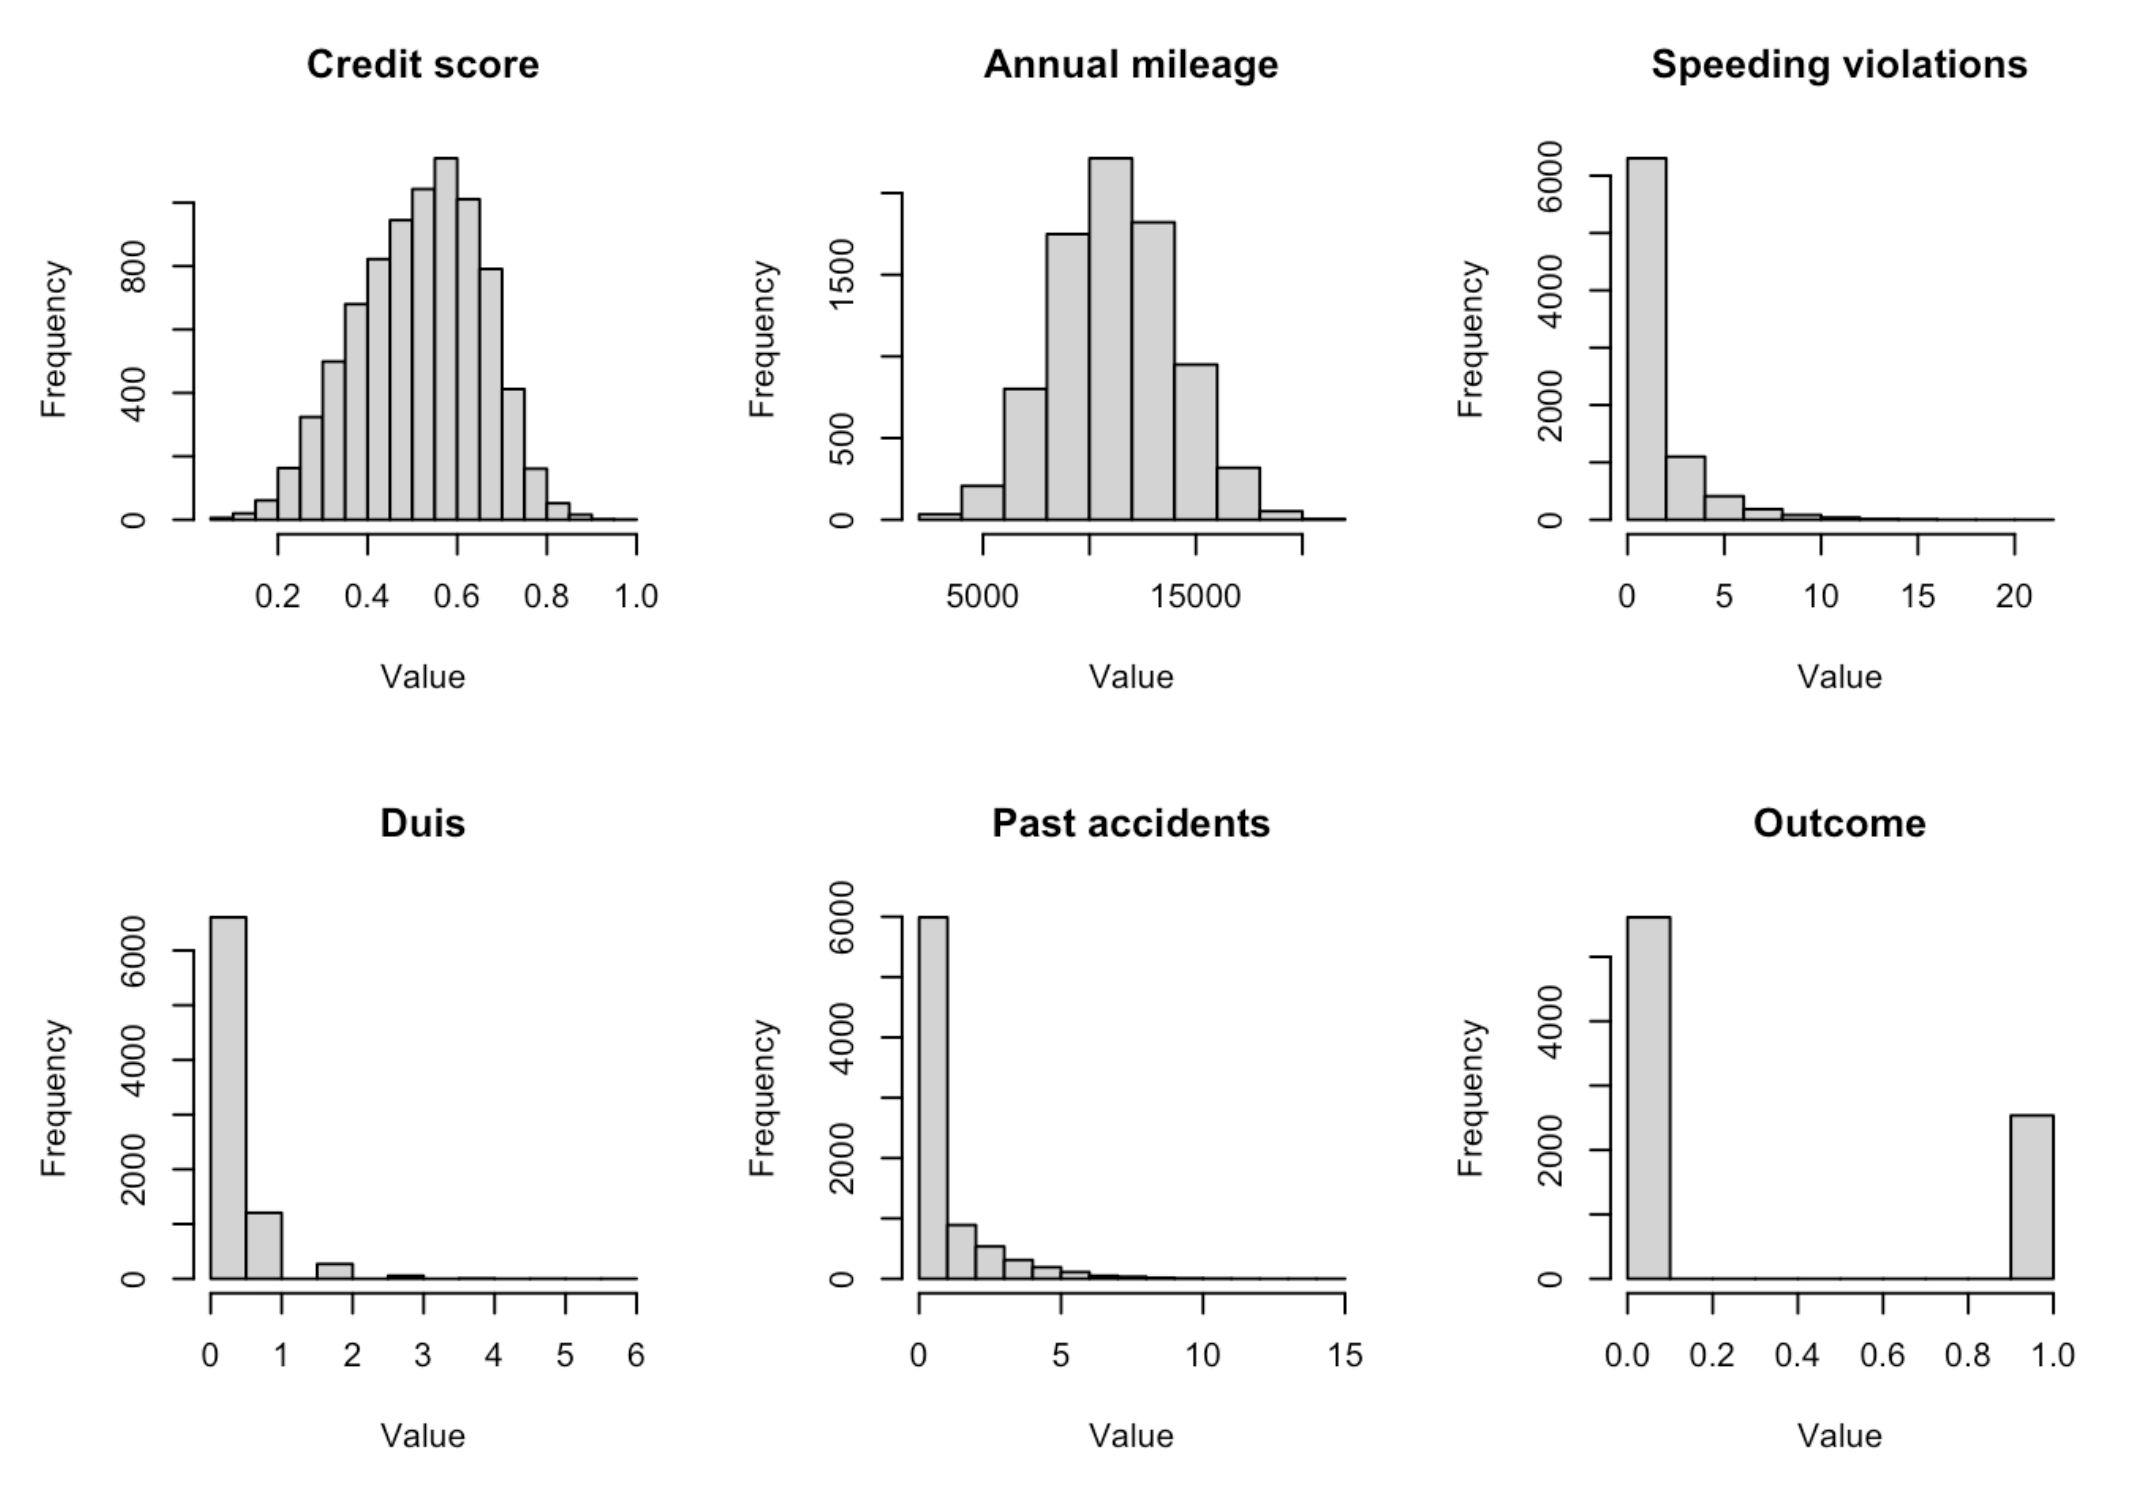
\includegraphics[scale=0.35]{eda.png}
    \caption{Histograms of the numerical variables.}
    \label{fig:histograms}
\end{figure}


\begin{figure}[!h]
    \centering
    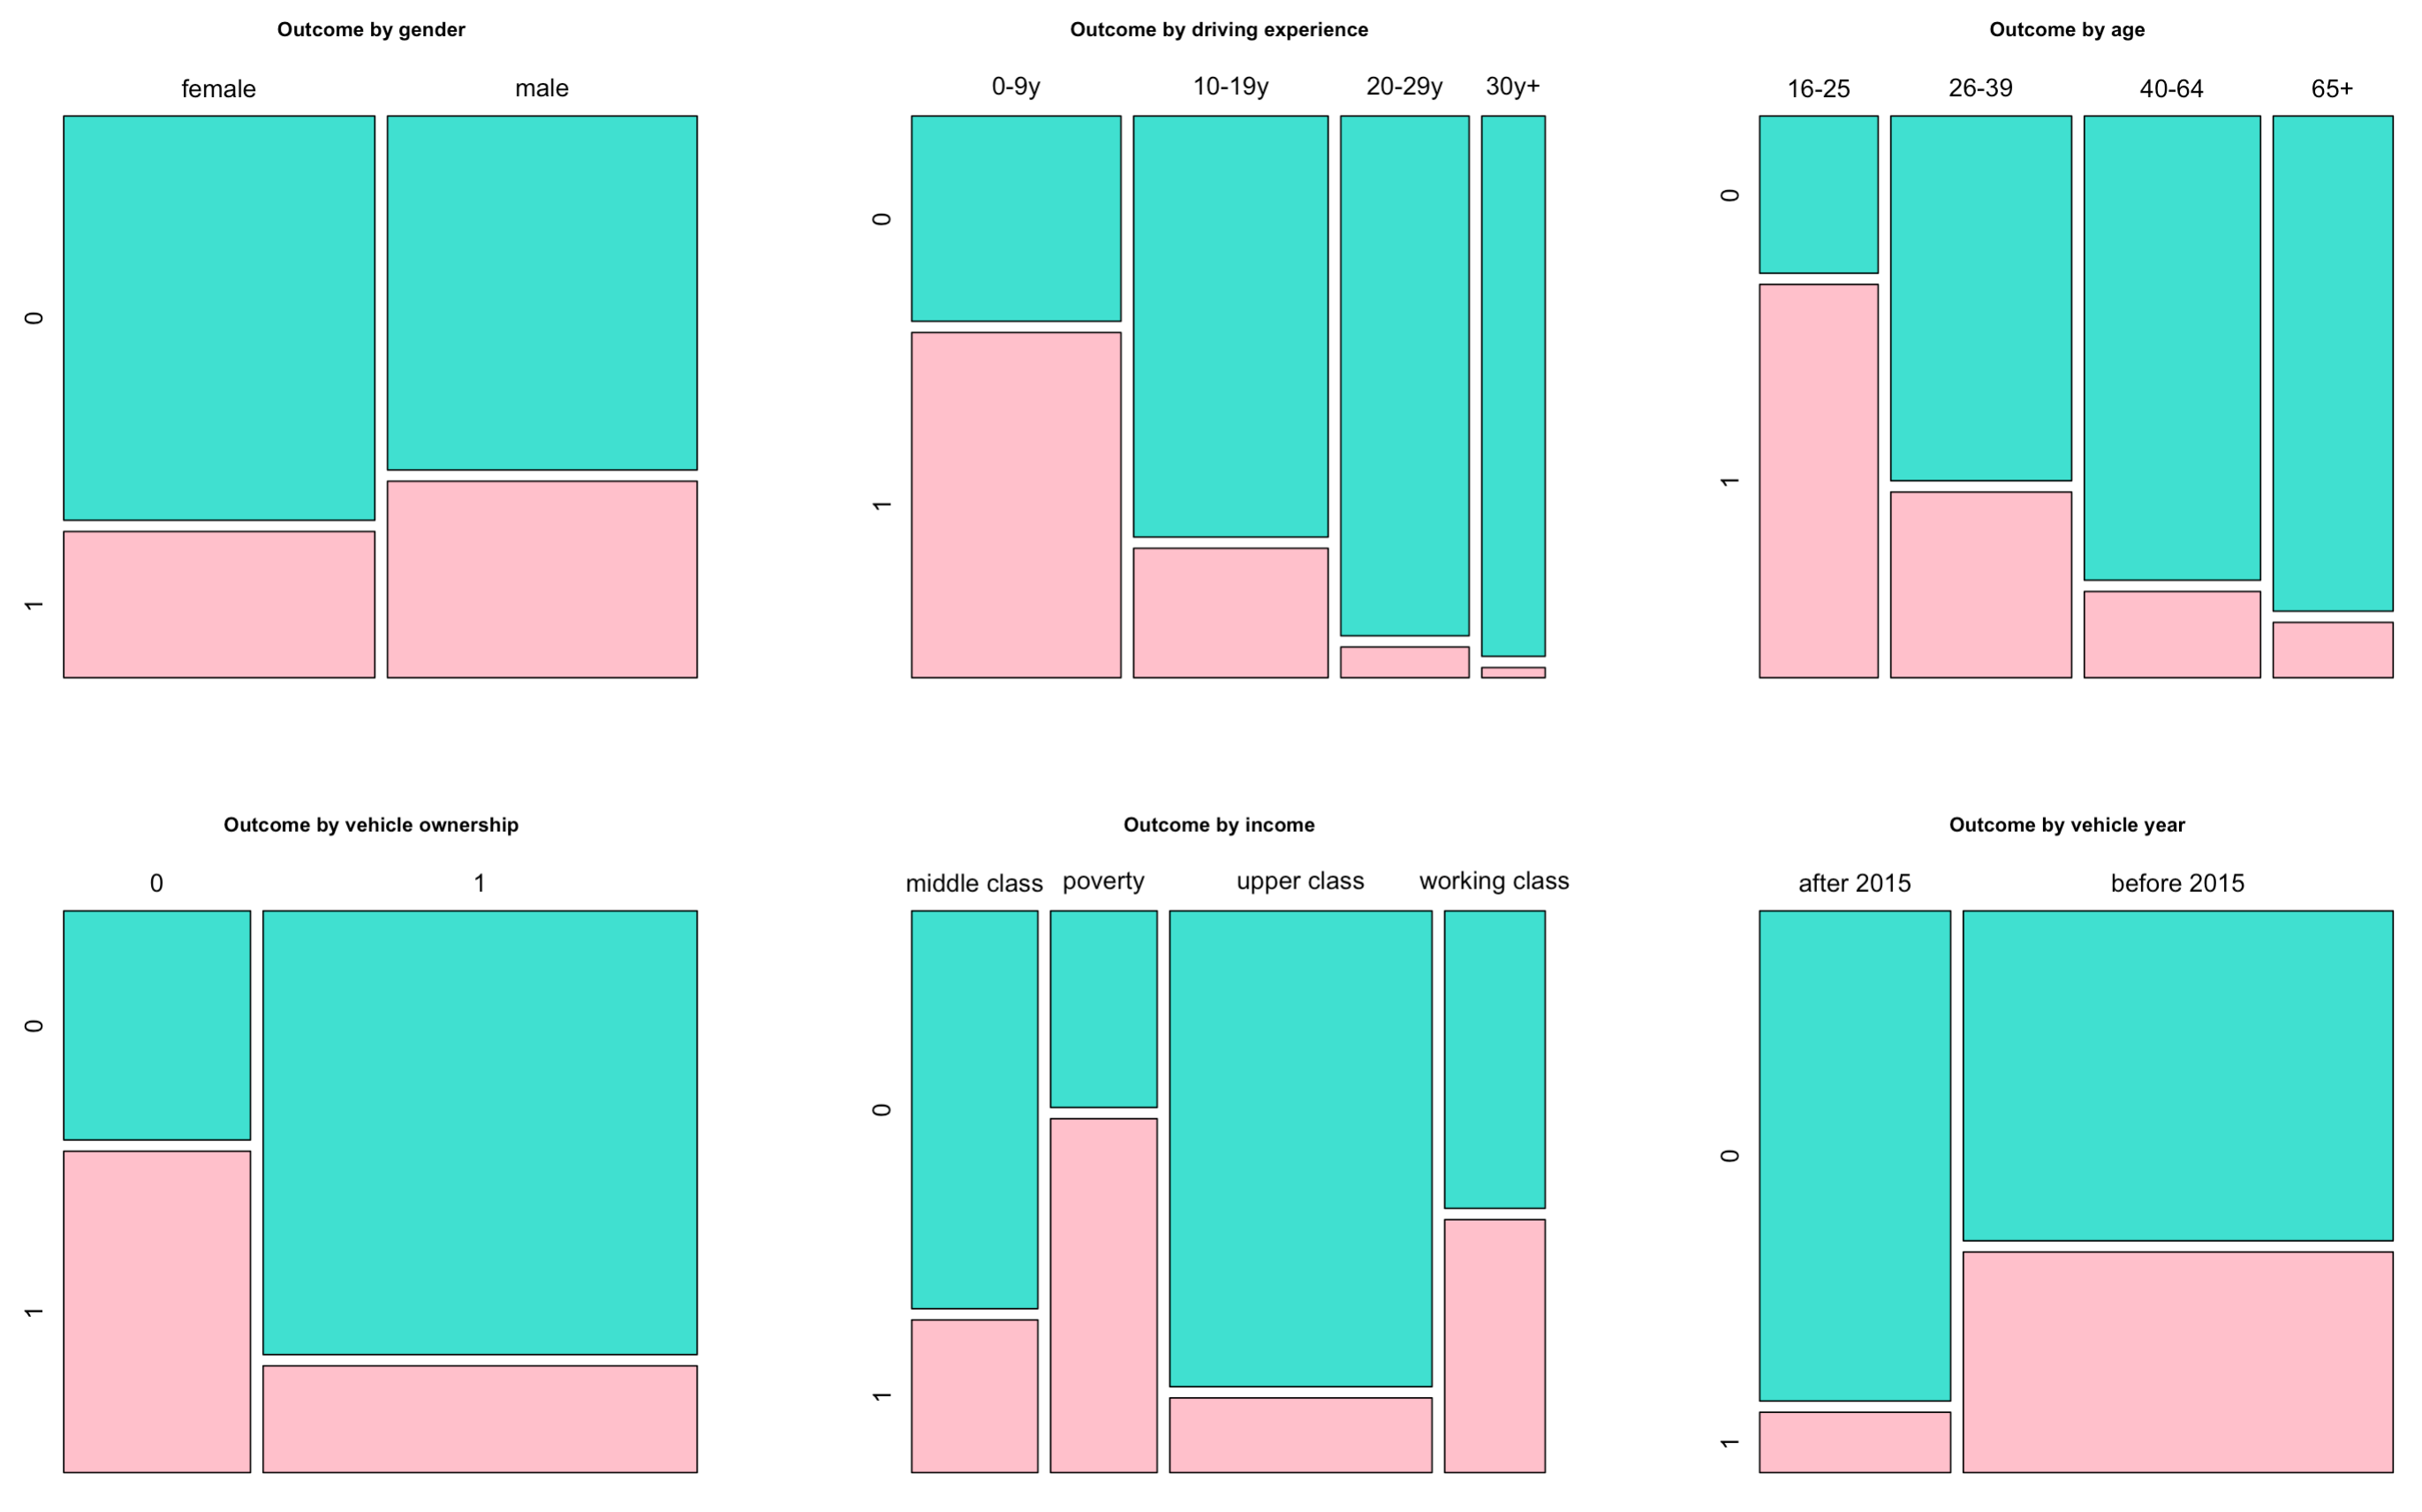
\includegraphics[scale=0.3]{eda-report.png}
    \caption{Value counts of categorical features with respect to the {\tt OUTCOME} value.}
    \label{fig:categorical-counts}
\end{figure}

\end{document}